\documentclass[11pt]{beamer}

\usetheme[progressbar=frametitle]{metropolis}
\usepackage{appendixnumberbeamer}
\usepackage{pgfpages}
%\setbeameroption{show notes on second screen}
  \setbeamertemplate{enumerate items}[square]

\usepackage{booktabs}

\usepackage{xcolor}

\newcommand{\link}[3][mLightBrown]{\href{#2}{\color{#1}{#3}}}%


\newcommand{\questionslide}[0]{
{\setbeamercolor{palette primary}{fg=black, bg=yellow}
\begin{frame}[standout]
    \raggedright
  Any questions? \\ \vspace{1cm}
  \raggedleft
  \dots{ } Remember -- Every question is useful!
\end{frame}
}}

\newcommand{\task}[1]{
   \begin{alertblock}
   {\centering \vspace{-1.5ex} \\ #1  \\ \vspace{-1.5ex} }
   \end{alertblock}
   }

\setbeamercolor{block title alerted}{%
    use={block title, alerted text},
    bg=yellow,
    fg=black
}

\definecolor{peppermint}{RGB}{75, 161, 115}
%\definecolor{peppermint}{RGB}{75, 161, 115}


\setbeamercolor{alerted text}{fg=peppermint , bg= black}

\usepackage{booktabs}
\usepackage[scale=2]{ccicons}

\usepackage{pgfplots}
\usepgfplotslibrary{dateplot}

\makeatletter 
\def\beamer@framenotesbegin{% at beginning of slide
    \usebeamercolor[fg]{normal text}
    \gdef\beamer@noteitems{}% 
    \gdef\beamer@notes{}% 
}
\makeatother


\usepackage{xspace}
\newcommand{\themename}{\textbf{\textsc{metropolis}}\xspace}

\title{Differences in Differences \\ (with a Time Series Detour)
}
\subtitle{Econ 140, Section 9 \\ MM Chapter 5}
% \date{\today}
\date{}
\author{Jonathan Old}

% \titlegraphic{\hfill\includegraphics[height=1.5cm]{logo.pdf}}

\begin{document}

\maketitle

\begin{frame}{Roadmap}
  \setbeamertemplate{section in toc}[sections numbered]
  \tableofcontents%[hideallsubsections]
\end{frame}




\section{IV revision}

\begin{frame}{Group work}

    \begin{itemize}
    
    
\item[\textit{Group 1:}] We are interested in the effect of being in the army on crime. We instrument being in the army with a lottery (\link{https://www.aeaweb.org/articles?id=10.1257/app.3.2.119}{paper})

\item[\textit{Group 2:}]  We are interested in the effect of protestant religion on economic growth. We instrument protestantism in a region with the distance to Wittenberg (\link{https://academic.oup.com/qje/article/124/2/531/1905076}{paper})

%\item[\textit{Group 2:}]  We are interested in the effect of income on conflict. We instrument income with rainfall (\link{https://www-journals-uchicago-edu.libproxy.berkeley.edu/doi/10.1086/421174}{paper})


\item[\textit{Group 3:}]  We are interested in the effect of air pollution on mortality. We instrument local air pollution with wind direction (\link{https://www.aeaweb.org/articles?id=10.1257/aer.20180279}{paper})



       \end{itemize}

\begin{enumerate}
    \item Relevance: Z must truly affect X
    \item Independence/Exogeneity: Z is as good as randomly assigned
    \item Exclusion restriction: The \textbf{only} way that Z affects Y is via X
\end{enumerate}

%\textbf{\alert{Your job: Discuss whether these three assumptions hold!!}}

 %  \begin{alertblock} {\centering \vspace{-1.5ex} \\ Your job: Discuss whether these three assumptions hold!  \\ \vspace{-1.5ex} } \end{alertblock}
    
    \task{Your job: Discuss whether these assumptions hold!}
   \end{frame}





\questionslide

\section{Time Series}

\begin{frame}{Why empirical microeconomists don't use time series}

Spurious correlations \alert{\link{https://www.tylervigen.com/spurious-correlations}{ here}.
}

Unsolicited financial advice \alert{\link{https://school.stockcharts.com/doku.php?id=chart_analysis:chart_patterns}{ here}}.


A great idea to lose your tuition fees is \alert{\link{https://twitter.com/i/status/1350854473598558213}{ here}}.

\end{frame}



\begin{frame}{Time series topics}
\begin{itemize}
\item Autoregressive and moving-average processes
\item Serial correlation (of the errors)
\item Unit roots
\item Trends
\item Detecting trend breaks
\item \dots
\end{itemize}

My prediction: Not the most important topic on the exam. But come to OH if you have questions or want to know more!

\end{frame}




\section{Motivation for DiD}

\begin{frame}{Motivation for Differences in Differences}
\begin{itemize}
    \item In the first part of the course, we talked about comparison between groups or other units (cross-sectional data)
    \item But we have also seen some comparisons over time: time-series data
    \item Both of these have very big and obvious problems, but we can use them \textbf{together} using (panel data) in a powerful tool: Differences-in-differences!
\end{itemize}
   
\end{frame}



\begin{frame}{How to get the causal effect of a treatment}

In 2021, UC Berkeley offered free mental health coachings to students with pre-existing mental health issues. We want to evaluate the effect of this policy and we collect a depression score (0-10) for all students at UC Berkeley. 

\begin{table}[]
\begin{tabular}{lcc}
\toprule
\textbf{}                        & \textbf{2020} & \textbf{2022} \\ \midrule
Free Mental Health: Treated      & 6          & 6          \\ \midrule
No Free Mental Health: Untreated & 4          & 5          \\ \bottomrule
\end{tabular}
\end{table}

We can do several comparisons:
\end{frame}







\begin{frame}{How to get the causal effect of a treatment II}


\begin{table}[]
\begin{tabular}{lcc}
\toprule
\textbf{}                        & \textbf{2020} & \textbf{2022} \\ \midrule
Free Mental Health: Treated      &           & 6          \\ \midrule
No Free Mental Health: Untreated &           &  5         \\ \bottomrule
\end{tabular}
\end{table}

We can do several comparisons:
\begin{itemize}[<+- | alert@+>]
\item Comparison 1: Compare treated and non-treated group after the intervention
\item Estimated treatment effect? $6-5=1$
\item Problems?
\item \textbf{Identifying assumption}: The average difference between groups is due to the treatment only. Without the treatment, the average outcome of the treated group would have been equal to the average outcome of the control group.
\end{itemize} 
\end{frame}






\begin{frame}{How to get the causal effect of a treatment III}


\begin{table}[]
\begin{tabular}{lcc}
\toprule
\textbf{}                        & \textbf{2020} & \textbf{2022} \\ \midrule
Free Mental Health: Treated      &    6       & 6          \\ \midrule
No Free Mental Health: Untreated &           &          \\ \bottomrule
\end{tabular}
\end{table}

We can do several comparisons:
\begin{itemize}[<+- | alert@+>]
\item Comparison 2: Compare treated group before and after the intervention
\item Estimated treatment effect? $6-6=0$
\item Problems?
\item Identifying assumption: The average difference across time is due to the treatment only. Without the treatment, the average outcome of the treated group would not have changed.
\end{itemize} 
\end{frame}





\begin{frame}{How to get the causal effect of a treatment: DiD}


\begin{table}[]
\begin{tabular}{lcc}
\toprule
\textbf{}                        & \textbf{2020} & \textbf{2022} \\ \midrule
Free Mental Health: Treated      &    6       & 6          \\ \midrule
No Free Mental Health: Untreated &    4       & 5        \\ \bottomrule
\end{tabular}
\end{table}

We can do several comparisons:
\begin{itemize}[<+- | alert@+>]
\item Comparison 3: Compare treated to untreated group, before and after the intervention. \textbf{Differences in differences!}
\item Estimated treatment effect? $(6-6)-(5-4)=(6-5)-(6-4)=-1$
\item Identifying assumption: Parallel trends: Without the treatment, the average increase in the outcome of the treated would have been the same as the average increase in the outcome of the untreated.
\end{itemize} 
\end{frame}


{\setbeamercolor{palette primary}{fg=black, bg=yellow}
\begin{frame}[standout]
    \raggedright
  Sidenote \\ \vspace{1cm}
  \raggedleft
  \dots{ } We can \textbf{NOT} observe the identifying assumption! We can find evidence for or against it, but we can never be sure!
\end{frame}}


\begin{frame}{How to get the causal effect of a treatment: DiD}


\begin{table}[]
\begin{tabular}{lcc}
\toprule
\textbf{}                        & \textbf{2020} & \textbf{2022} \\ \midrule
Free Mental Health: Treated      &    6       & 6          \\ \midrule
No Free Mental Health: Untreated &    4       & 5        \\ \bottomrule
\end{tabular}
\end{table}

We can calculate the DiD estimate in two ways (here: superscripts stand for treatment/control group, subscripts denote unit $i$ and time $t\in\{0,1\}$)
\begin{align*}
DiD &=E[\underbrace{\left(Y_{i 1}^T-Y_{i 0}^T\right)}_{\text{Change for treated}}-\underbrace{\left(Y_{i 1}^C-Y_{i 0}^C\right)}_{\text{Change for untreated}}]  \\
 &=E[\underbrace{\left(Y_{i 1}^T-Y_{i 1}^C\right)}_{\text{After-difference}}-\underbrace{\left(Y_{i 0}^T-Y_{i 0}^C\right)}_{\text{Before-difference}}] 
\end{align*}


\end{frame}






\begin{frame}{DiD and Potential Outcomes}
Let us look at the second one in more detail:
$$
\begin{aligned}
DiD &=E[\left(Y_{i 1}^T-Y_{i 1}^C\right)-\left(Y_{i 0}^T-Y_{i 0}^C\right)] \\
&= \underbrace{\left(E[Y_{i 1}^T]-E[Y_{i 1}^C]\right)}_{\text{After-difference}}-\underbrace{\left(E[Y_{i 0}^T]-E[Y_{i 0}^C]\right)}_{\text{Before-difference}} 
\end{aligned}
$$

Compare this with out formula for selection bias (in time period 1):
$$
\begin{aligned}
\Delta &= E[Y_{i1}^T]-E[Y_{i1}^C] \\ 
&= \underbrace{E[\text{Y}^T_{i1}(1) - \text{Y}^T_{i1}(0)]}_{\text{ATT}} + \underbrace{\left(  E[\text{Y}^T_{i1}(0)] - E[\text{Y}^C_{i1}(0)] \right)}_{\text{Selection Bias}}
\end{aligned}
$$

\end{frame}










\begin{frame}{DiD and Potential Outcomes}
Let us look at the second one in more detail:
$$
\begin{aligned}
DiD &=E[\left(Y_{i 1}^T-Y_{i 1}^C\right)-\left(Y_{i 0}^T-Y_{i 0}^C\right)] \\
&= \underbrace{  \left( {\color{red} E[Y_{i 1}^T]-E[Y_{i 1}^C] } \right)}_{\text{After-difference}}-\underbrace{\left( {\color{TolLightBlue} E[Y_{i 0}^T]-E[Y_{i 0}^C]}\right)}_{\text{Before-difference}} 
\end{aligned}
$$

Compare this with out formula for selection bias (at $t=1$):
$$
\begin{aligned}
\Delta &= {\color{red} E[Y_{i1}^T]-E[Y_{i1}^C] } \\ 
&= \underbrace{E[\text{Y}^T_{i1}(1) - \text{Y}^T_{i1}(0)]}_{\text{ATT}} + \underbrace{\left(  {\color{TolLightBlue} E[\text{Y}^T_{i1}(0)] - E[\text{Y}^C_{i1}(0)]}  \right)}_{\text{Selection Bias}}
\end{aligned}
$$
So DiD=ATT if the before-difference is equal to the selection bias in period 1: If the treatment group hadn't gotten the treatment (potential outcome = 0), the difference to the control group would have been the same as in period 0.


\end{frame}





\begin{frame}{Parallel trends assumption}

\begin{figure}
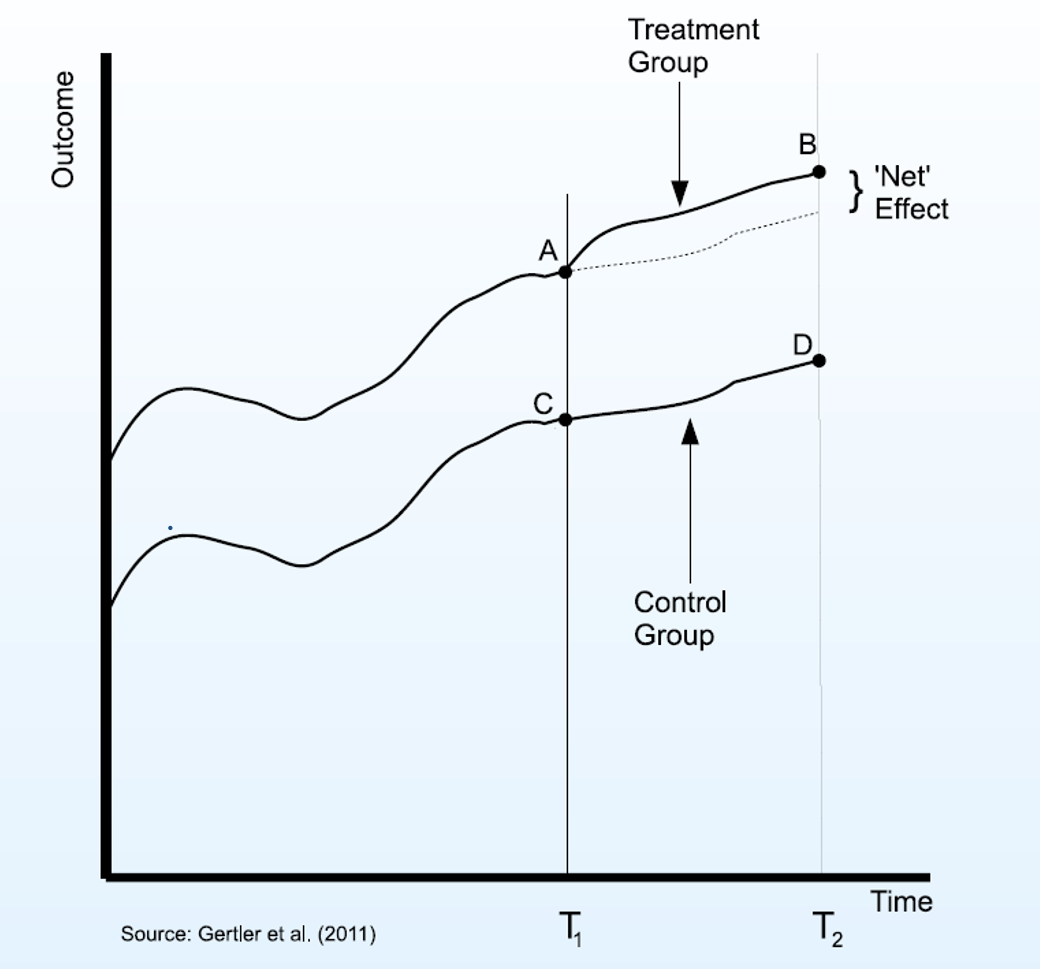
\includegraphics[width=0.8\textwidth]{figures/did1.png}
\end{figure}

\end{frame}




\begin{frame}{(Potential) violation of a parallel trends assumption}

\begin{figure}
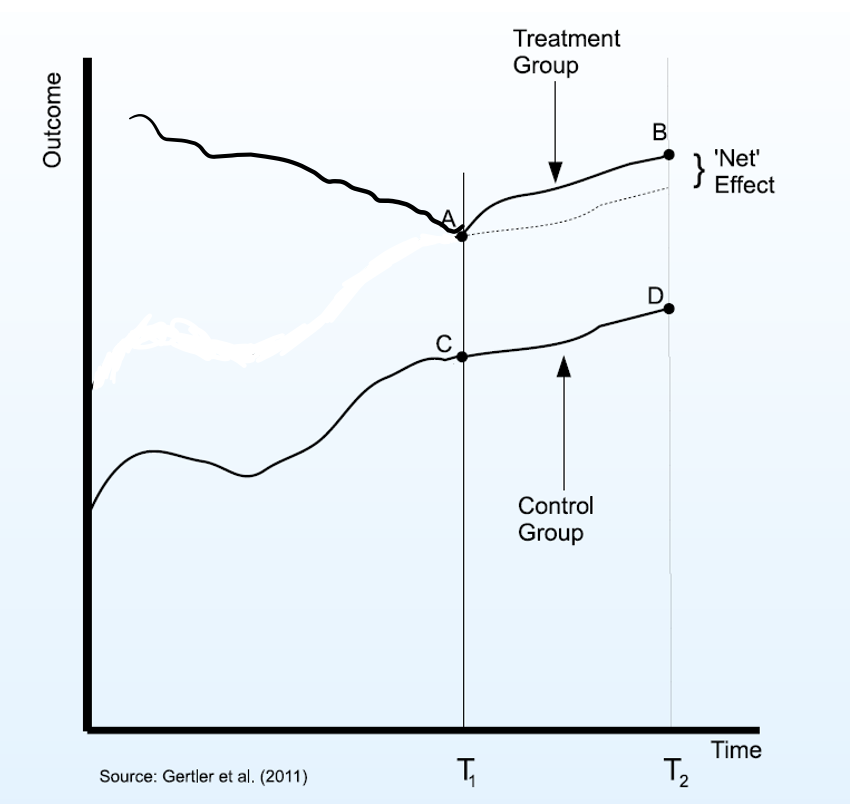
\includegraphics[width=0.8\textwidth]{figures/did2.png}
\end{figure}

\end{frame}




\begin{frame}{Estimating DiD with regressions}
We can set up a simple linear regression to estimate a  DiD model:
$$
Y_{i t}=\alpha+\beta \text { Treated }_i+\gamma \text { Post }_t+\delta \text { Treated }_i \cdot \text { Post }_t+u_{i t}
$$


\begin{table}[]
\begin{tabular}{lcc}
\toprule
\textbf{}                        & \textbf{2020} & \textbf{2022} \\ \midrule
Free Mental Health: Treated      &        &          \\ \midrule
No Free Mental Health: Untreated &    $\alpha$       &         \\ \bottomrule
\end{tabular}
\end{table}


\end{frame}




\begin{frame}{Estimating DiD with regressions}
We can set up a simple linear regression to estimate a  DiD model:
$$
Y_{i t}=\alpha+\beta \text { Treated }_i+\gamma \text { Post }_t+\delta \text { Treated }_i \cdot \text { Post }_t+u_{i t}
$$


\begin{table}[]
\begin{tabular}{lcc}
\toprule
\textbf{}                        & \textbf{2020} & \textbf{2022} \\ \midrule
Free Mental Health: Treated      &          &          \\ \midrule
No Free Mental Health: Untreated &    $\alpha$       & $\alpha + \gamma$        \\ \bottomrule
\end{tabular}
\end{table}


\end{frame}






\begin{frame}{Estimating DiD with regressions}
We can set up a simple linear regression to estimate a  DiD model:
$$
Y_{i t}=\alpha+\beta \text { Treated }_i+\gamma \text { Post }_t+\delta \text { Treated }_i \cdot \text { Post }_t+u_{i t}
$$


\begin{table}[]
\begin{tabular}{lcc}
\toprule
\textbf{}                        & \textbf{2020} & \textbf{2022} \\ \midrule
Free Mental Health: Treated      &    $\alpha + \beta$       &         \\ \midrule
No Free Mental Health: Untreated &    $\alpha$       & $\alpha + \gamma$        \\ \bottomrule
\end{tabular}
\end{table}


\end{frame}





\begin{frame}{Estimating DiD with regressions}
We can set up a simple linear regression to estimate a  DiD model:
$$
Y_{i t}=\alpha+\beta \text { Treated }_i+\gamma \text { Post }_t+\delta \text { Treated }_i \cdot \text { Post }_t+u_{i t}
$$



\begin{table}[]
\begin{tabular}{lcc}
\toprule
\textbf{}                        & \textbf{2020} & \textbf{2022} \\ \midrule
Free Mental Health: Treated      &    $\alpha + \beta$       & $\alpha + \beta + \gamma + \delta$          \\ \midrule
No Free Mental Health: Untreated &    $\alpha$       & $\alpha + \gamma$        \\ \bottomrule
\end{tabular}
\end{table}


\end{frame}










\begin{frame}{Estimating DiD with regressions}
We can set up a simple linear regression model to get the DiD estimate:
$$
Y_{i t}=\alpha+\beta \text { Treated }_i+\gamma \text { Post }_t+\delta \text { Treated }_i \cdot \text { Post }_t+u_{i t}
$$
\begin{table}[]
\begin{tabular}{lcc}
\toprule
\textbf{}                        & \textbf{2020} & \textbf{2022} \\ \midrule
Free Mental Health: Treated      &    6       & 6          \\ \midrule
No Free Mental Health: Untreated &    4       & 5        \\ \bottomrule
\end{tabular}
\end{table}

With our data, we would get:
\begin{itemize}
\item $\alpha = 4$
\item $\beta = 2$
\item $\gamma = 1$
\item $\delta = -1$

\end{itemize}


\end{frame}




\questionslide



\section{Rainfall IV: Checking relevance with DiD}


\begin{frame}{Rainfall and Income}
You are hired by the Government of Ghana to study the impact of income on the level of education. Using data on rural villages, you estimate the following population regression using OLS:
$$
E d u c_i=\beta_0+\beta_1 \text { Income }_i+\beta_2 \text { Pop }_i+\beta_3 \text { School }_i+\beta_4 \text { Age }_i+u_i
$$
where Educ$_i$ is average years of formal education in the village, Income$_i$ is average annual income per capita in the village, Pop$_i$ is the number of village residents, School$_i$ is the number of schools in the village, and Age$_i$ is the average age of the village population.

Explain what econometric problem is likely to arise that leads to biased and inconsistent estimates as a result of including Income as a regressor in the education regression as is done above.
\end{frame}



\begin{frame}{IV regression}
We want to know the effect of income on education and estimate
$$
E d u c_i=\beta_0+\beta_1 \text { Income }_i+\beta_2 \text { Pop }_i+\beta_3 \text { School }_i+\beta_4 \text { Age }_i+u_i
$$


You learn from Ghana's Minister of Agriculture that the country's citizens derive the bulk of their income from agriculture. As a result, you cleverly infer that average annual rainfall (Rainfall) may be a good instrument for income. You recall from your econometrics course that an instrument can be used in a procedure called Two Stage Least Squares that is designed to solve this econometric problem. Describe carefully the first of the two stages.


\end{frame}




\begin{frame}{Checking Relevance with DiD}

You want to check the Minister's suggestion that rainfall has an impact on incomes in Ghana. You have information on average annual incomes in 1996 and 1997 for two regions: the "coastal region," which had the same precipitation level in both years, and the "hill region," which experienced a $30 \%$ increase in rainfall. Comparing 1996 and 1997, income in the coastal region fell from 124 to 104, while income in the hill region fell from 98 to 96 . You also recall from your econometrics course that this situation might represent a "natural" or "quasi" experiment, allowing you to estimate the "treatment effect" of rainfall. Perform a difference in differences analysis of the effect of rainfall on average income. Summarize the analysis in a table.


\end{frame}

\begin{frame}{DiD summary}

$$
\begin{array}{|c|c|c|c|}
\hline \text { Region } & \text { Rainfall } & 1996 & 1997 \\
\hline \text { Coast (control) } & \text { No change } & 124 & 104 \\
\hline \text { Hill (treatment) } & +30 \% & 98 & 96 \\
\hline
\end{array}
$$

This is equivalent to estimating:
$$I_{it}=\beta_0+\beta_1 G_i+\beta_2 D_t+\beta_3 G_i \times D_t+u_i $$

where 
 $G_i=1$ if village is in Hills and $G_i=0$ if village is on the Coast; $D_t=1$ if year is 1997 and $D_t=0$ if year is 1996. The differences in differences estimate of the rainfall effect is the OLS of $\beta_3$.


\end{frame}




\end{document}
